\documentclass[11pt]{article}
\usepackage[toc,page]{appendix}
\usepackage{amsmath, amssymb}
\usepackage[utf8]{inputenc}
\usepackage[T1]{fontenc}
\usepackage[style=apa,backend=biber]{biblatex}
%\usepackage{biblatex}
\addbibresource{references.bib}
\usepackage{graphicx}
\usepackage{tikz}
\usetikzlibrary{automata,positioning,shapes.geometric, arrows.meta, fit, backgrounds, calc, chains}
\graphicspath{./images/Easy_Pictures/SMR_MULT_Repackaging}%\usepackage{kpfonts}
\usepackage{float}
\usepackage[margin=1in]{geometry}
\usepackage{cancel}
\usepackage{epsfig}
\usepackage{tikz-3dplot}
\usepackage{darkmode}
\usepackage{dirtytalk}
\usepackage{longtable,booktabs,array}
\usepackage{calc} % for calculating minipage widths
\usepackage[utf8]{inputenc}
\usepackage[T1]{fontenc}
\usepackage{xcolor}
\usepackage{listings}


\usepackage{etoolbox}
\usepackage{hyperref}
\hypersetup{
    colorlinks=true,
    linkcolor=blue,
    filecolor=magenta,      
    urlcolor=cyan,
    pdftitle={Hermeneutic Calculator},
    citecolor=blue,
    }


\urlstyle{same}

\lstdefinestyle{htmlStyle}{
    language=HTML,
    basicstyle=\ttfamily\small,
    keywordstyle=\color{blue}\bfseries,
    commentstyle=\color{gray}\itshape,
    stringstyle=\color{red},
    breaklines=true,
    frame=single,
    numbers=left,
    numberstyle=\tiny\color{gray},
    columns=fullflexible,
}
\lstdefinelanguage{HTML}{
  keywords={<!DOCTYPE, html, head, title, body, h1, h2, h3, p, div, span, a, img, ul, li, table, tr, td, th, style, link, script},
  sensitive=true,
  comment=[l]{//},
  morecomment=[s]{/*}{*/},
  morestring=[b]',
  morestring=[b]"
}
\lstset{style=htmlstyle, language=html}
% Updated to explicitly pass the language option
%\lstinputlisting[style=htmlstyle, language=html]{./html/example.html}
%\usepackage{tocloft}

% Optional: define some custom colors
\definecolor{sliceRed}{RGB}{225,224,91} % matching "varyellow" from your code
\definecolor{linkYellow}{RGB}{255,215,0}  % a golden yellow
\tdplotsetmaincoords{70}{110}

\title{Addition Strategies: Rearranging to Make Bases (RMB)}
\author{Compiled by: Theodore M. Savich}


\begin{document}
\maketitle
\subsection*{Transcript}
Video from \textcite{Carpenter1999}. Strategy descriptions and examples adapted from \textcite{HackenbergCourseNotes}. 
\begin{itemize}
\item \textbf{Teacher:} Lucy is eight fish. She buys five more fish. How many fish will Lucy have then?
\item \textbf{Sarah:}  13. 
\item \textbf{Teacher:} How'd you get 13? 
\item \textbf{Sarah:} Well, because eight plus two is ten, but then two plus three is five. And she wants to buy five more fish. So you take care of two, and you need to add three more. And so I add three more, and you get 13.
\end{itemize}

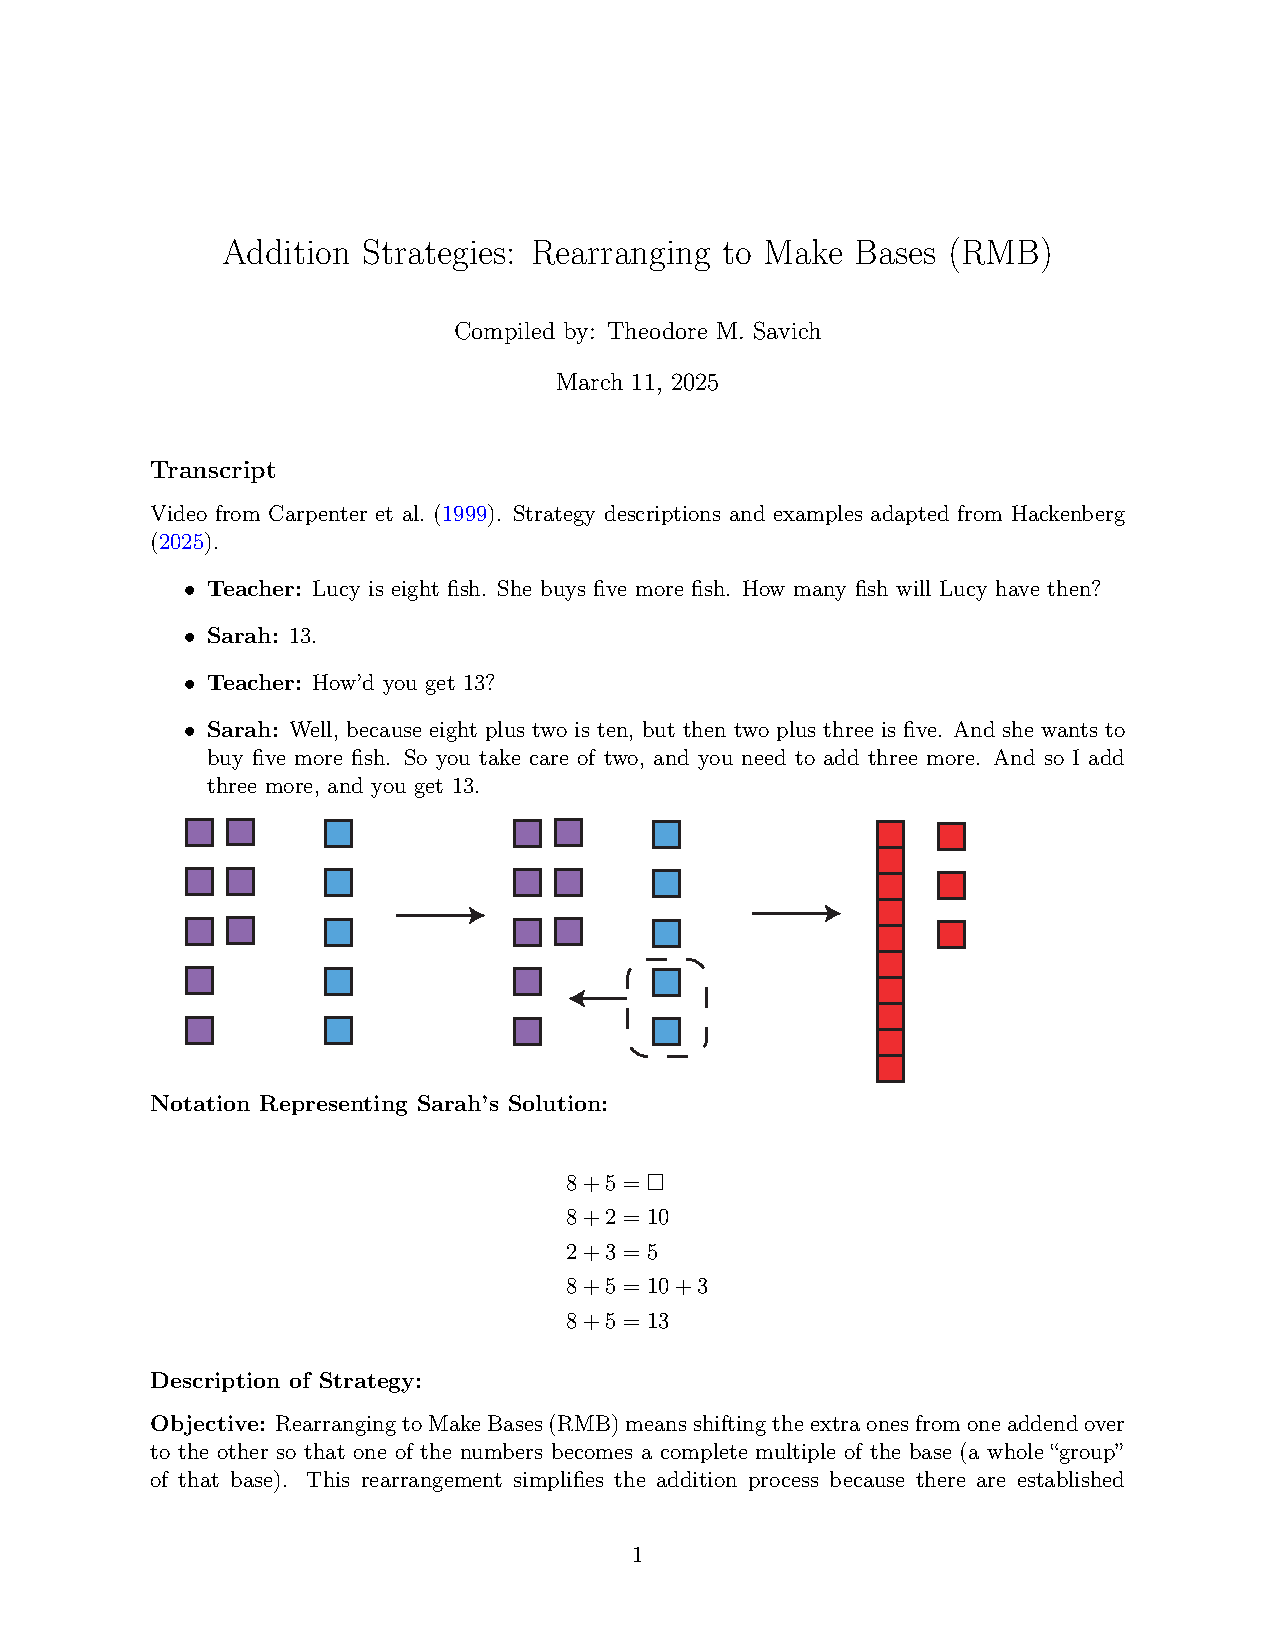
\includegraphics[width=.8\textwidth]{images/Easy_Pictures/SAR_ADD_RMB/PDF/SAR_ADD_RMB.pdf}

\noindent \textbf{Notation Representing Sarah's Solution:}

\begin{align*}
8 + 5 &= \Box \\
8+2 &= 10\\
2+3 &= 5\\
8+5&= 10 + 3\\
8+5 &= 13
\end{align*}

\subsubsection*{Description of Strategy:}

 \textbf{Objective:} Rearranging to Make Bases (RMB) means shifting the extra ones from one addend over to the other so that one of the numbers becomes a complete multiple of the base (a whole ``group'' of that base). This rearrangement simplifies the addition process because there are established patterns for adding an exact multiple of the base. In other words, when you add a full group of base units to a number, the ones digit stays the same while only the digit representing the base (like the tens place) increases.
   

\subsection*{Rearranging to Make Bases (RMB)}

\subsubsection*{Description of Strategy}
\begin{itemize}
    \item \textbf{Objective:} Make one of the addends a whole number of bases by moving ones from the other addend.
    \item \textbf{Example:} \(8 + 5\)
    \begin{itemize}
        \item Move 2 ones from 5 to 8 to make 10.
        \item Remaining ones in the second addend: \(5 - 2 = 3\).
        \item Add the adjusted numbers: \(10 + 3 = 13\).
    \end{itemize}
\end{itemize}

\subsubsection*{Automaton Type}
\textbf{Pushdown Automaton (PDA)}: Needed to handle digits and to remember the number of ones moved via the stack.

\subsubsection*{Formal Description of the Automaton}

We define the PDA as the 7-tuple
\[
M = (Q,\Sigma,\Gamma,\delta,q_{0/accept},Z_0,F)
\]
where
\begin{itemize}
    \item \(Q = \{q_{0/accept},\, q_1,\, q_2,\, q_3,\, q_4,\, q_5\}\) is the finite set of states.
    \item \(\Sigma = \{0,1,2,3,4,5,6,7,8,9,+\}\) is the input alphabet (suitable for representing addends).
    \item \(\Gamma = \{Z_0\} \cup \{x \mid x \in \mathbb{N}\}\) is the stack alphabet, where:
        \begin{itemize}
            \item \(Z_0\) is the initial (bottom) stack symbol.
            \item A symbol \(x\) represents the number of ones moved.
        \end{itemize}
    \item \(q_{0/accept}\) is the start state, which is also the accept state.
    \item \(Z_0\) is the initial stack symbol.
    \item \(F = \{q_{0/accept}\}\) is the set of accepting states.
\end{itemize}

The transition function 
\[
\delta: Q \times (\Sigma \cup \{\varepsilon\}) \times \Gamma \to \mathcal{P}(Q \times \Gamma^*)
\]
is defined by the following key transitions:
\begin{enumerate}
    \item \(\delta\Bigl(q_{0/accept},\, \text{``}A,B\text{''},\, Z_0\Bigr) = \{(q_1,\, Z_0)\}\) \quad (Read inputs \(A\) and \(B\)).
    \item \(\delta(q_1,\, \varepsilon,\, Z_0) = \{(q_2,\, Z_0)\}\) \quad (Determine the ones digits of \(A\) and \(B\)).
    \item \(\delta(q_2,\, \varepsilon,\, Z_0) = \{(q_3,\, Z_0)\}\) \quad (Compute the number of ones needed to make \(A\) a full base).
    \item \(\delta(q_3,\, \varepsilon,\, Z_0) = \{(q_4,\, k\,Z_0)\}\) \quad (If \(B\) has at least \(k\) ones, push \(k\) onto the stack).
    \item \(\delta(q_4,\, \varepsilon,\, k) = \{(q_5,\, k)\}\) \quad (Move \(k\) ones from \(B\) to \(A\) and adjust the addends).
    \item \(\delta(q_5,\, \varepsilon,\, k) = \{(q_{0/accept},\, Z_0)\}\) \quad (Add the adjusted numbers, output the result, and pop \(k\) from the stack).
\end{enumerate}

\subsubsection*{Automaton Diagram for RMB}

The following TikZ picture arranges the 6 states on a circle, with \(q_{0/accept}\) serving as both the start and accept state.

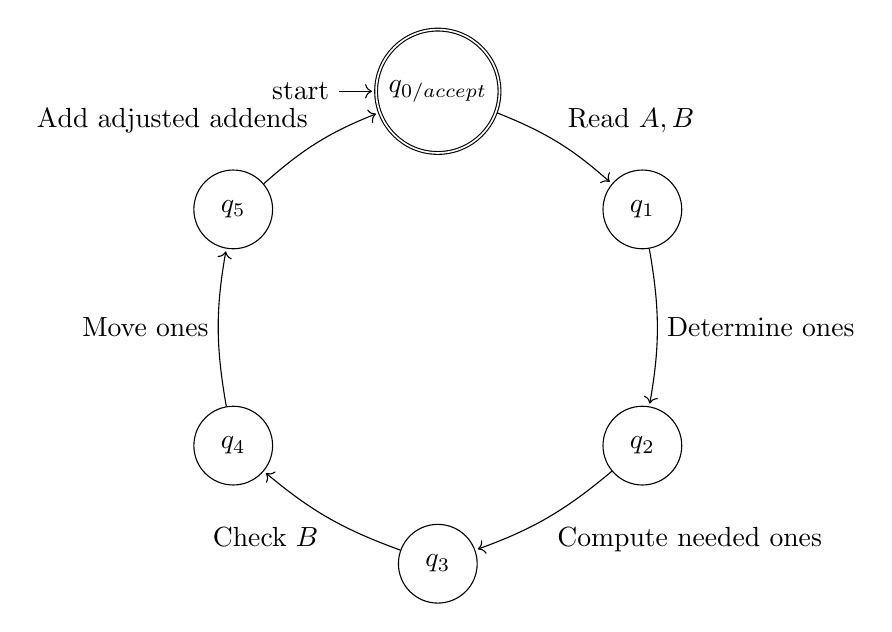
\begin{tikzpicture}[
    shorten >=1pt,
    on grid,
    auto,
    every state/.style={minimum size=1cm}
]
    % Define radius and start angle
    \def\radius{3cm}
    \def\startangle{90}
    % There are 6 states; angular increment is 360/6 = 60 degrees.
    \def\incangle{60}
    
    % Nodes arranged on a circle
    \node[state, initial, accepting] (q0) at (\startangle:\radius) {$q_{0/accept}$};
    \node[state] (q1) at ({\startangle-\incangle}:\radius) {$q_1$};
    \node[state] (q2) at ({\startangle-2*\incangle}:\radius) {$q_2$};
    \node[state] (q3) at ({\startangle-3*\incangle}:\radius) {$q_3$};
    \node[state] (q4) at ({\startangle-4*\incangle}:\radius) {$q_4$};
    \node[state] (q5) at ({\startangle-5*\incangle}:\radius) {$q_5$};
    
    % Transitions between states
    \path[->]
        (q0) edge[bend left=10] node {Read \(A,B\)} (q1)
        (q1) edge[bend left=10] node {Determine ones} (q2)
        (q2) edge[bend left=10] node {Compute needed ones} (q3)
        (q3) edge[bend left=10] node {Check \(B\)} (q4)
        (q4) edge[bend left=10] node {Move ones} (q5)
        (q5) edge[bend left=10] node {Add adjusted addends} (q0);
\end{tikzpicture}

\subsubsection*{HTML Implementation}
\lstinputlisting[style=htmlStyle, language=html]{./new_html/SAR_ADD_RMB.html}

\printbibliography
\end{document}